
        \documentclass[tikz]{standalone}
        \usepackage{tikz}
        \usetikzlibrary{matrix}
        \begin{document}
        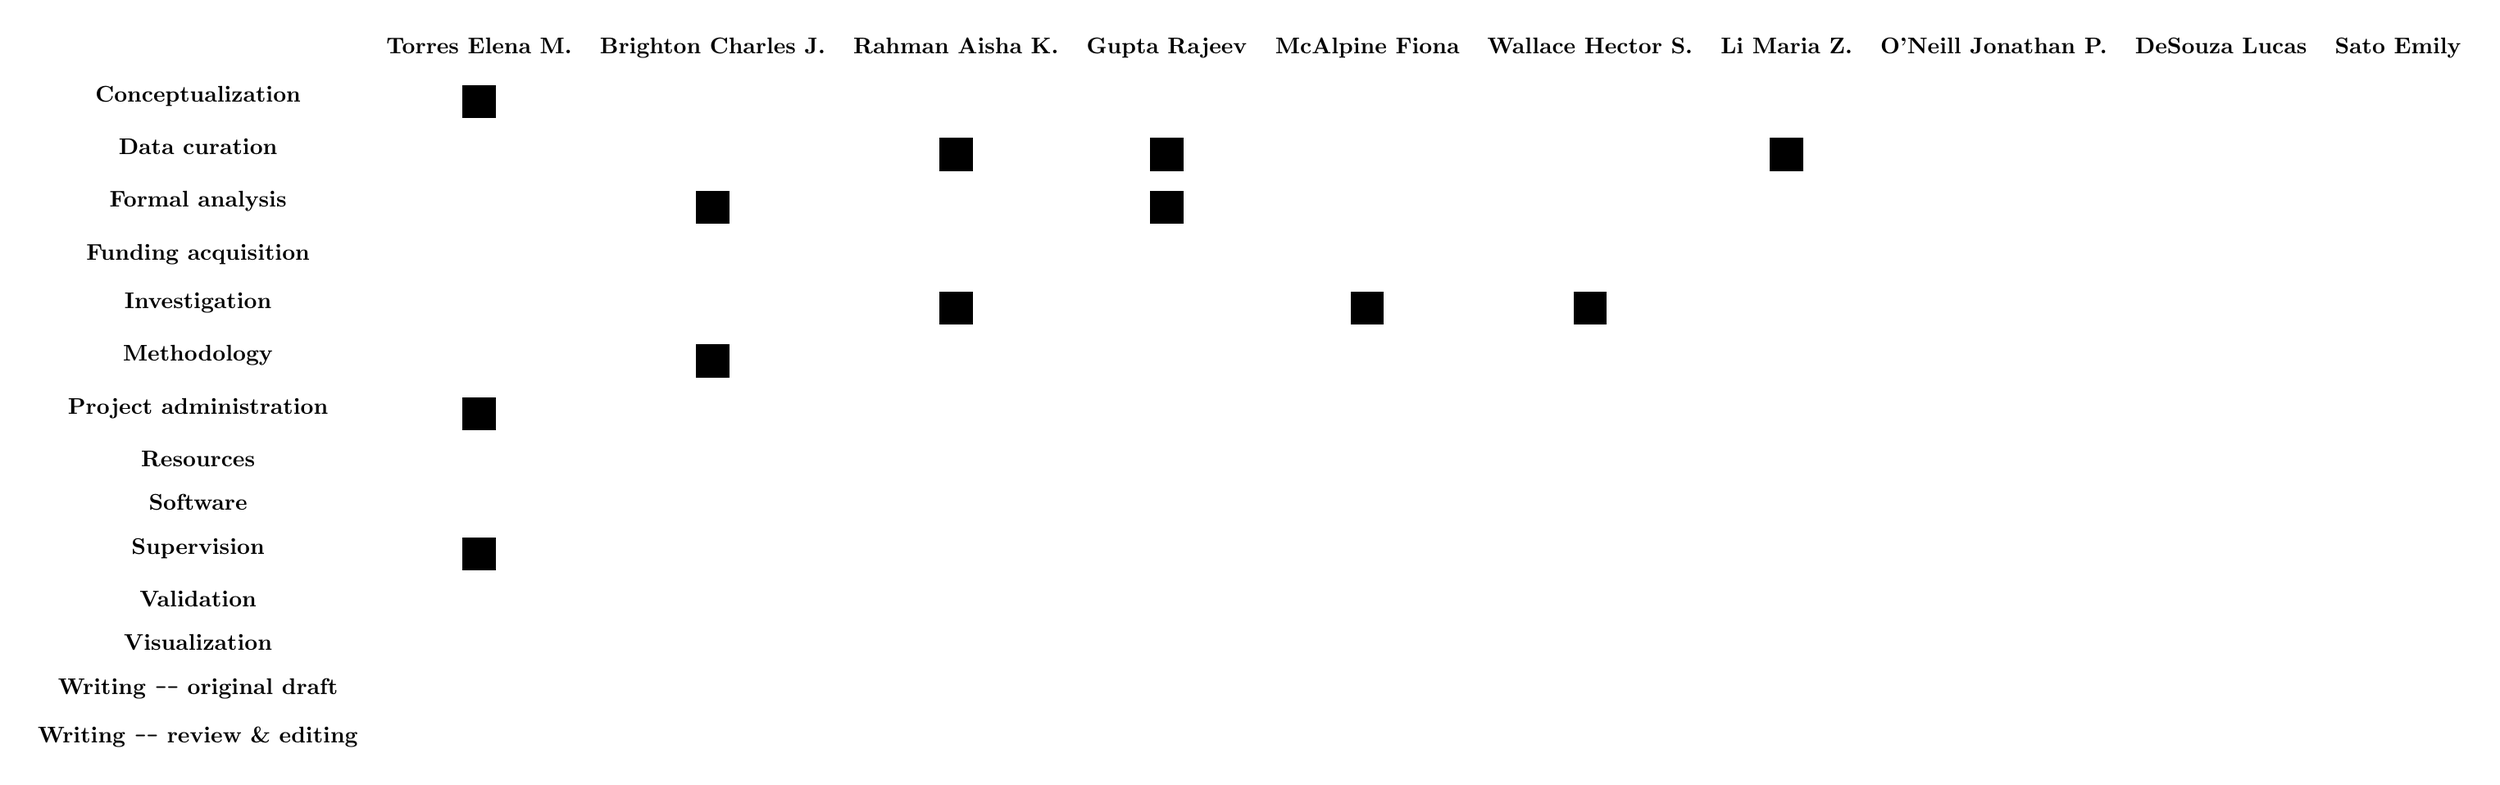
\begin{tikzpicture}
  \tikzset{rolestyle/.style={draw, minimum size=5mm, fill=black, anchor=center}}
  % Define the matrix with empty cells
  \matrix (contribmatrix) [matrix of nodes, nodes in empty cells, column sep=2mm, row sep=2mm] {
  & \textbf{Torres Elena M.} & \textbf{Brighton Charles J.} & \textbf{Rahman Aisha K.} & \textbf{Gupta Rajeev} & \textbf{McAlpine Fiona} & \textbf{Wallace Hector S.} & \textbf{Li Maria Z.} & \textbf{O'Neill Jonathan P.} & \textbf{DeSouza Lucas} & \textbf{Sato Emily} \\
  \textbf{Conceptualization} & |[rolestyle]| &  &  &  &  &  &  &  &  &  \\
  \textbf{Data curation} &  &  & |[rolestyle]| & |[rolestyle]| &  &  & |[rolestyle]| &  &  &  \\
  \textbf{Formal analysis} &  & |[rolestyle]| &  & |[rolestyle]| &  &  &  &  &  &  \\
  \textbf{Funding acquisition} &  &  &  &  &  &  &  &  &  &  \\
  \textbf{Investigation} &  &  & |[rolestyle]| &  & |[rolestyle]| & |[rolestyle]| &  &  &  &  \\
  \textbf{Methodology} &  & |[rolestyle]| &  &  &  &  &  &  &  &  \\
  \textbf{Project administration} & |[rolestyle]| &  &  &  &  &  &  &  &  &  \\
  \textbf{Resources} &  &  &  &  &  &  &  &  &  &  \\
  \textbf{Software} &  &  &  &  &  &  &  &  &  &  \\
  \textbf{Supervision} & |[rolestyle]| &  &  &  &  &  &  &  &  &  \\
  \textbf{Validation} &  &  &  &  &  &  &  &  &  &  \\
  \textbf{Visualization} &  &  &  &  &  &  &  &  &  &  \\
  \textbf{Writing \texttt{--} original draft} &  &  &  &  &  &  &  &  &  &  \\
  \textbf{Writing \texttt{--} review \& editing} &  &  &  &  &  &  &  &  &  &  \\
};
\end{tikzpicture} 
        \end{document}
        